\documentclass{beamer}
\usetheme{Warsaw}
\usecolortheme{beaver}
\usepackage{graphicx}

\title{Git introduction for beginners}
\subtitle{Get off, mercurial users}
\author[Keruspe \and Judu]{Marc-Antoine Perennou \and Julien Durillon}
\institute[CC]{Clever Cloud -- http://www.clever-cloud.com/}
\date{}

\begin{document}

\begin{frame}[plain]
    \titlepage
\end{frame}

\begin{frame}{Who we are}
      Marc-Antoine Perennou - 
\includegraphics[width=80px,height=30px]{logo-cc.png} \\[0.5cm]
      \hrule \hfill \\[0.5cm]
      Marc-Antoine@Perennou.com \\
      marc-antoine.perennou@clever-cloud.com \\[0.5cm]
      \hrule \hfill \\[0.5cm]
      @Keruspe on twitter and identi.ca \\
      http://github.com/Keruspe
\end{frame}
\begin{frame}{Who we are}
      Julien Durillon - 
\includegraphics[width=80px,height=30px]{logo-cc.png} \\[0.5cm]
      \hrule \hfill \\[0.5cm]
      julien.durillon@gmail.com \\
      julien.durillon@clever-cloud.com \\[0.5cm]
      \hrule \hfill \\[0.5cm]
      @juuduu on twitter \\
      http://github.com/judu
\end{frame}

\begin{frame}{The (D)VCS concept}
    \begin{itemize}
        \item What is a Version Control System?
        \pause
        \item Why must you use one?
        \pause
        \item Why should you consider using or switching to a Distributed VCS?
    \end{itemize}
    \begin{minipage}{0.4\textwidth}
    \begin{flushleft}
    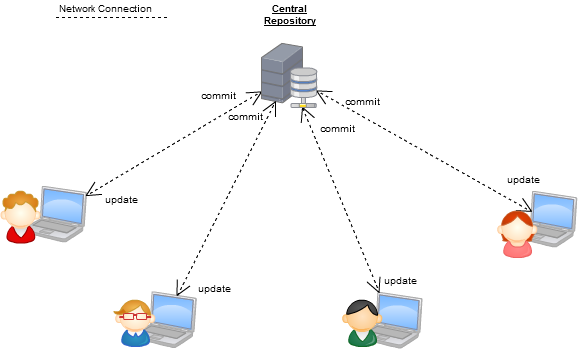
\includegraphics[width=\textwidth]{VCS.png}
    \end{flushleft}
    \end{minipage}
    \hfill\vrule\hfill
    \begin{minipage}{0.4\textwidth}
    \begin{flushright}
    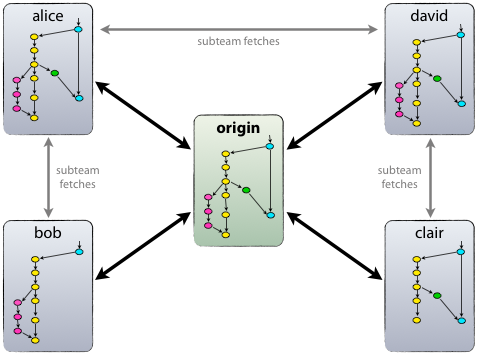
\includegraphics[width=\textwidth]{DVCS.png}
    \end{flushright}
    \end{minipage}\\[0.2cm]
    \begin{minipage}{0.2\textwidth}
    \begin{flushright}
    VCS
    \end{flushright}
    \end{minipage}\hfill
    \begin{minipage}{0.5\textwidth}
    \begin{center}
    VS
    \end{center}
    \end{minipage}\hfill 
    \begin{minipage}{0.2\textwidth}
    \begin{flushleft}
    DVCS
    \end{flushleft}
    \end{minipage}
\end{frame}

\begin{frame}{The origin of Git}
    
\includegraphics[width=60pt,height=30pt]{git-scm-logo.png}
    \begin{itemize}
        \item The creation of git
        \begin{itemize}
            \item Linux development constraints (Too many developers, thousands per year)
            \item First release: 2005
        \end{itemize}
        \pause
        \item The origin of its name
        \pause
        \item The evolution/complexification and usage simplification of git
    \end{itemize}
\end{frame}

\begin{frame}{Creating a repository}
    One command: git init\\
    This command creates the basic files needed by git into a subdirectory named ".git" \\
    \ \\
    \ \\
    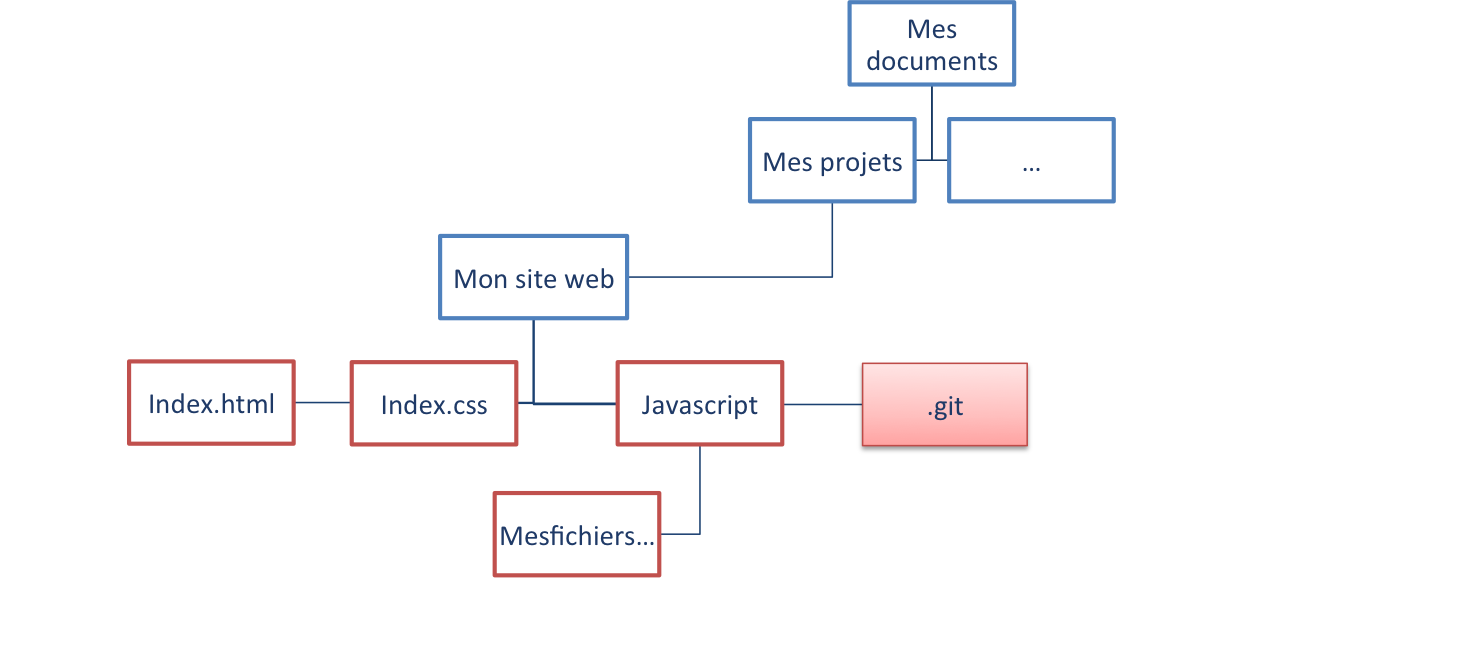
\includegraphics[width=250pt,height=110pt]{fileinit.png}
\end{frame}

\begin{frame}{But\dots what's in .git?}
\begin{itemize}
   \item Full repository\pause
   \item \emph{i.e.}:
      \begin{itemize}
         \item full commit history
         \item all objects since the project beginning
         \item all local and shared branches
         \item all tags
         \item registered remotes
         \item hooks (useful for CI)
      \end{itemize}
\end{itemize}
\end{frame}

\begin{frame}{But\dots what's a commit?}
   \begin{itemize}
      \item Author \onslide<2->{ -- The one who wrote the code}
      \item Commiter \onslide<3->{ -- The one who created the commit object}
      \item Parent \onslide<4->{ -- The commit(s) before this one}
      \item Tree \onslide<5->{ -- The top tree object of the commited state}
      \item Message \onslide<6->{ -- Why the commit was done}
   \end{itemize}
 
   \begin{center}
      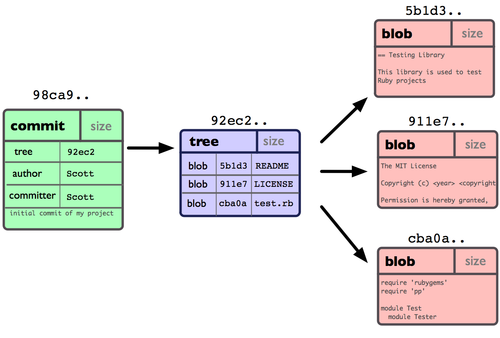
\includegraphics[width=0.5\textwidth]{commit-object.png}
   \end{center}
\end{frame}

\begin{frame}{Basic usage}
    6 mandatory commands : \\
    \begin{itemize}
        \item git init
        \item git clone
        \item git add
        \item git commit
        \item git push
        \item git pull
    \end{itemize}
    With those commands (and eventually git remote), you can act with git at least like you acted with SVN (for example)
\end{frame}

\begin{frame}{Git server side}
    \begin{itemize}
        \item Introduction to github
        \pause
        \item Demonstration: sharing this presentation on github
        \pause
        \item For your company: gitolite
        \pause
        \item Git with non-git backend
    \end{itemize}
\end{frame}

\begin{frame}{Some useful basics}
    \begin{itemize}
        \item Explanations on the tracking system (diff VS file)
        \pause
        \item Configuration
        \pause
        \item Editing the last commit
        \pause
        \item Cleaning a working tree
    \end{itemize}
\end{frame}

\begin{frame}{Branching}
    Three commands: \\
    \begin{itemize}
        \item git branch
        \item git checkout
        \item git merge
    \end{itemize}
    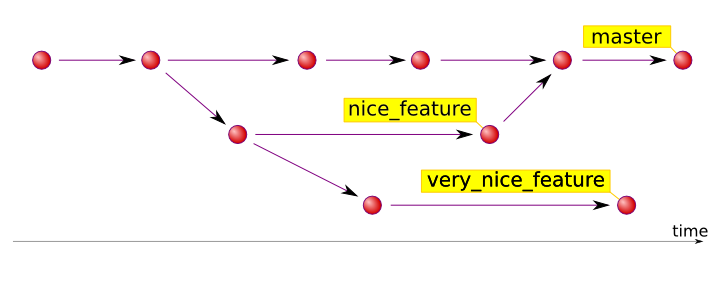
\includegraphics[width=300pt,height=130pt]{branches.png}
\end{frame}

\begin{frame}{But\dots what's a branch?}
   \begin{itemize}
      \item Just a reference\dots\pause
      \item on a commit\dots\pause
      \item that is updated by the \emph{commit} command.
   \end{itemize}
   \begin{center}
   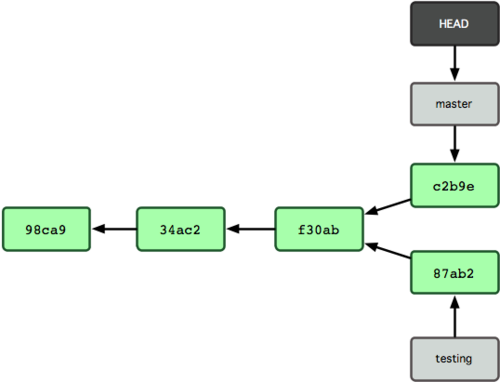
\includegraphics[width=0.5\textwidth]{branches-inside.png}
   \end{center}
\end{frame}

\begin{frame}{Advanced usage}
    \begin{itemize}
        \item Rebasing with git rebase / git pull -{}-rebase
        \pause
        \item Rearranging your commits
        \pause
        \item Patching with git format-patch and git am
        \pause
        \item Backporting with git cherry-pick for maintainance
        \pause
        \item Debugging with git bisect
        \pause
        \item Tagging releases
        \pause
        \item Blaming colleagues
    \end{itemize}
\end{frame}

\begin{frame}{Demos}
   \begin{itemize}
      \item Failing merge
      \pause
      \item Successfull fast-forwarding merge
      \pause
      \item Backporting changes
   \end{itemize}
\end{frame}

\begin{frame}{Questions?}
\end{frame}

\end{document}
